\documentclass[12pt]{article}
\usepackage{graphicx}
\usepackage[margin=1in]{geometry}
\usepackage{tikz}
\usepackage{listings}
\usepackage{color} % Required for custom colors
\usepackage{courier} % Set the font for listing as Courier
% Define custom colors
\definecolor{mygreen}{rgb}{0,0.6,0}
\definecolor{mygray}{rgb}{0.5,0.5,0.5}
\definecolor{mymauve}{rgb}{0.58,0,0.82}

% Define the MATLAB code style
\lstdefinestyle{mystyle}{
    backgroundcolor=\color{white},
    basicstyle=\footnotesize\ttfamily,
    commentstyle=\color{mygreen},
    keywordstyle=\color{blue},
    numberstyle=\tiny\color{mygray},
    numbers=left,
    numbersep=5pt,
    showspaces=false,
    showstringspaces=false,
    showtabs=false,
    tabsize=2,
    fontadjust=true,
    columns=fullflexible,
    keepspaces=true
}
\lstset{style=mystyle}

\begin{document}

\title{ELCT 432: Problem Assignment \#6}
\author{Jacob C. Vaught}
\date{11-06-2023}
\maketitle

\subsection*{Directions}
Develop a MATLAB code for generating a random message signal \( x[n] \) where its autocorrelation function is \( R[k] = \text{sinc}^2\left(\frac{1}{4} k\right) \) where \( k \) is an integer. 

\noindent (Hint: Generate a process where autocorrelation is Dirac (i.e., the Power Spectral Density (PSD) has equal power on all frequency components, (you can use \texttt{randn(1,N)} where \( N \) is a large number, e.g., 100000)) and exploit the Wiener-Khinchin Theorem (i.e., \( S_{YY}(f) = F\{R_{YY}(\tau)\} \) where \( S_{YY}(f) = |H(f)|^2 S_{XX}(f) \)).

\subsection*{MATLAB Code Explanation}
A white noise signal with uniform power across all frequencies is generated using MATLAB's \texttt{randn} function. This signal passes through a filter whose magnitude response in the frequency domain is designed to match the square root of the desired PSD, which is based on the signal's autocorrelation function.

\subsubsection*{Filter Design}
The filter's frequency response is determined by taking the square root of the PSD derived from the autocorrelation function. Given that the autocorrelation is defined as \( R[k] = \text{sinc}^2\left(\frac{k}{4}\right) \), the corresponding PSD will have a rectangular shape due to the Fourier Transform properties of the sinc function. Thus, the filter's shape in the frequency domain is a box (rectangular), and due to the squaring operation, the PSD will become triangular.

\newpage
\section*{Results and Discussion}

\subsection*{Autocorrelation Functions}
The theoretical autocorrelation function is a sinc squared function, which when sampled gives rise to the empirical autocorrelation function. These functions are plotted and compared to confirm the accuracy of the signal generation process.

\begin{figure}[h]
\centering
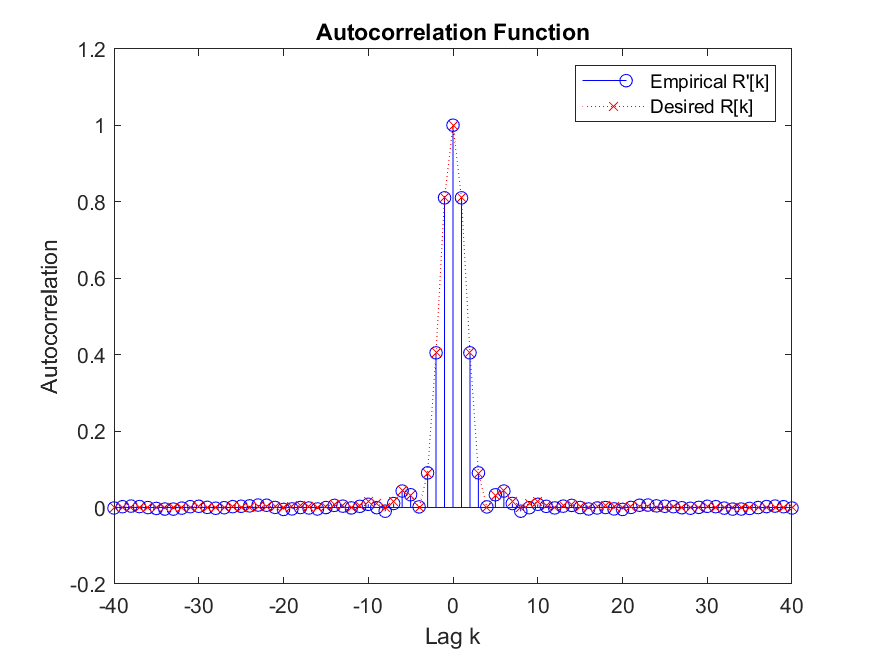
\includegraphics[width=0.8\textwidth]{Autocorrelation_Function.png}
\caption{Comparison between the theoretical and empirical autocorrelation functions.}
\label{fig:autocorr}
\end{figure}

As shown in Figure \ref{fig:autocorr}, the theoretical and empirical autocorrelation functions exhibit a strong resemblance, affirming the correctness of the generated message signal.

\subsection*{Power of the Message Signal}
The power of the message signal can be computed as the mean square value of the time-domain signal, which should theoretically be equal to \( R[0] \), the autocorrelation at zero lag. This is expected since the power of the signal is the area under the PSD, which corresponds to the peak of the sinc function in the autocorrelation representation.
\subsection*{Power Spectral Density}

When a random signal, which can be represented by white noise, is passed through a filter with a rectangular magnitude response, the output signal takes on the characteristics of the filter's frequency response. A rectangular filter shapes the signal's autocorrelation function into a sinc function due to the inverse Fourier transform of the rectangle.

The Power Spectral Density (PSD) is defined as the Fourier transform of the autocorrelation function of the signal. For a rectangular filter, this autocorrelation function is a sinc function due to the filtering process:

\[
R(\tau) = \text{sinc}(\tau)
\]

However, we are interested in the power of the signal, which is proportional to the square of the amplitude. Therefore, we consider the squared sinc function:

\[
R^{2}(\tau) = \text{sinc}^{2}(\tau)
\]

The PSD is then given by the Fourier transform of \( R^{2}(\tau) \), which due to the properties of Fourier transforms, results in the convolution of two rectangular functions:

\[
\mathcal{F}\{\text{sinc}^2(t)\} = (\text{rect} * \text{rect})(f)
\]

where \( * \) denotes the convolution operation, and \( \text{rect}(f) \) is the rectangle function in the frequency domain, which is the Fourier transform of the sinc function. The result of this convolution is a triangular function, which explains the triangular shape of the PSD when a signal is passed through a rectangular filter.

The triangular PSD indicates that the signal contains most of its power around the center frequency and gradually tapers off as we move away from the center, resembling the shape of a triangle. Therefore, when observing the PSD of our filtered signal, we expect to see a triangular distribution of power across frequencies.

\begin{figure}[h]
\centering
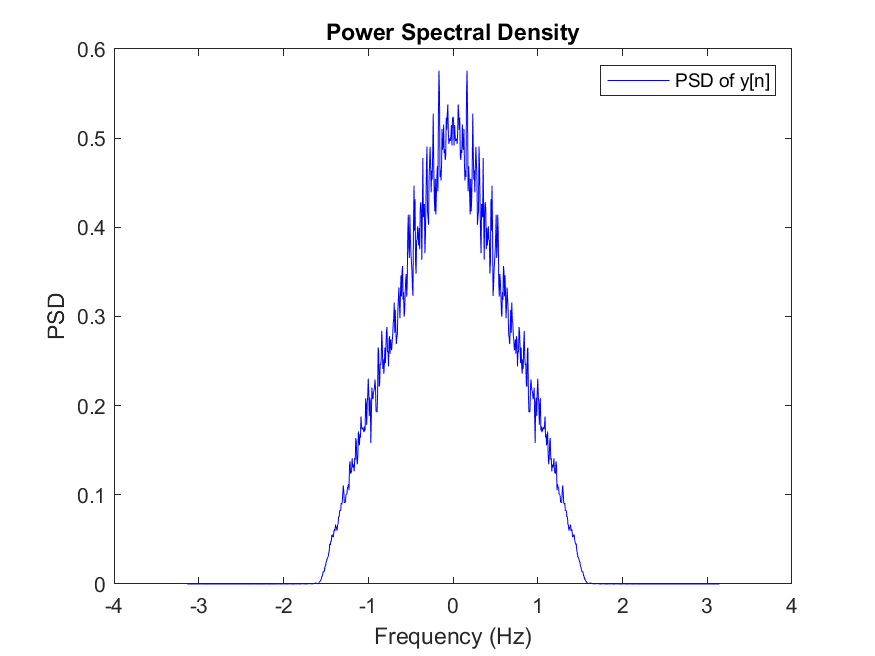
\includegraphics[width=0.7\textwidth]{Power_Spectral_Density.png}
\label{fig:psd}
\end{figure}

Figure \ref{fig:psd} depicts the PSD of the message signal. The triangular shape is consistent with the theoretical expectations from the filter design.
\begin{figure}[h]
\centering
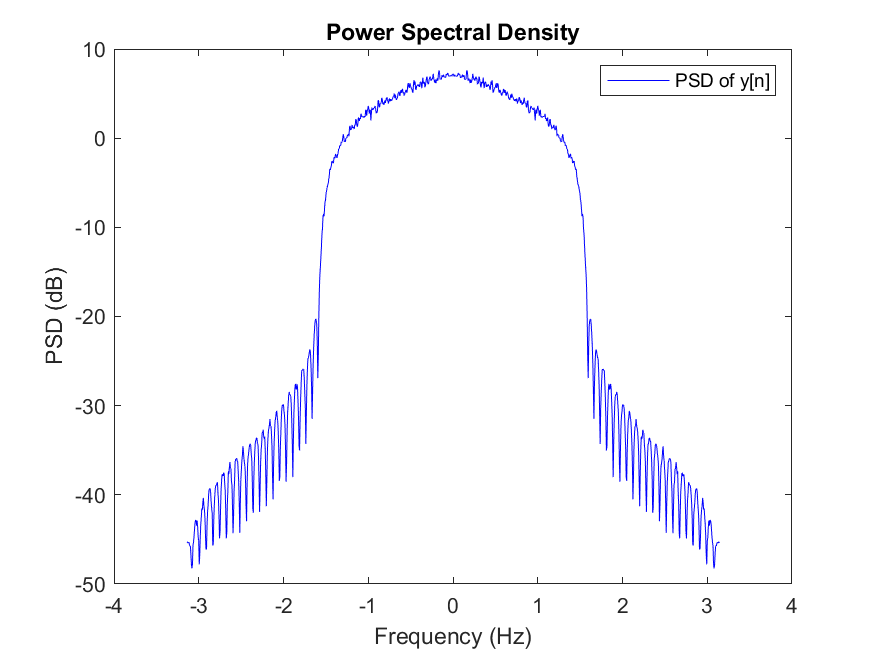
\includegraphics[width=0.7\textwidth]{Power_Spectral_Density_dB.png}
\label{fig:psdDb}
\end{figure}

\newpage
\subsection*{Bandwidth in DSB-SC Modulation}
In DSB-SC modulation, the bandwidth of the transmitted signal is ideally twice the highest frequency component of the message signal, which would be 3 Hz for a perfect rectangular filter. However, the sinc function extends infinitely, implying an infinite bandwidth. In practice, the bandwidth is finite and determined by the filter's cutoff frequency, with the understanding that there is a trade-off between bandwidth and sidelobe suppression.
\newpage
\section*{MATLAB Code}
\lstinputlisting[language=Matlab]{PA6_432.m}

\end{document}
